\documentclass[times,twoside,watermark]{rilab}
\usepackage[colorinlistoftodos]{todonotes}
\usepackage{float}
\usepackage{lipsum}
\setlength\headheight{30.15244pt} %% just to make warning go away. Adjust the value after looking into the warning.
% \rhead{{\color{blue}\rule{1cm}{1cm}}}

\rhead{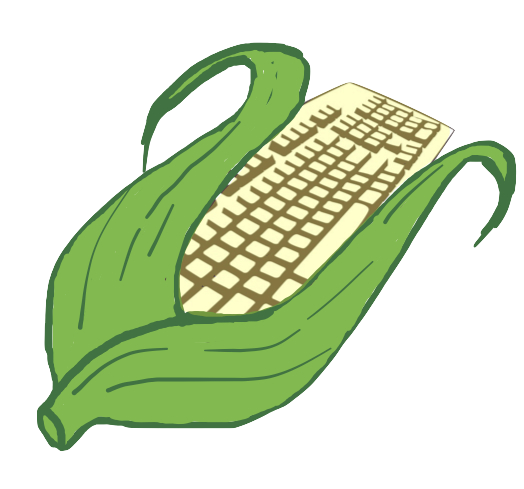
\includegraphics[width=1cm]{Figures/cornkey.png}}


% Please give the surname of the lead author for the running footer
\leadauthor{Andrews}

\begin{document}

\title{Ross-Ibarra Lab bioRxiv template}
\shorttitle{RILAB Template}

% Use letters for affiliations, numbers to show equal authorship (if applicable) and to indicate the corresponding author
\author[1,\Letter]{Felix Andrews}

\affil[1]{Dept of Plant Sciences, University of California, 1 Shields Ave, Davis, CA 95616, USA}

\maketitle

%TC:break Abstract
%the command above serves to have a word count for the abstract
\begin{abstract}
\lipsum[1-1]
\end {abstract}
%TC:break main
%the command above serves to have a word count for the abstract

\begin{keywords}
corn | corn | corn | more corn
\end{keywords}

\begin{corrauthor}
%\texttt{r.henriques{@}ucl.ac.uk}
f.andrews\at rilab.org
\end{corrauthor}

\section*{Introduction}
\lipsum[1-4]

\section*{Results}
\lipsum[3-5]

Just for kicks here's a citation \citep{Gustafsson2016}. And a reference to a supplement \cref{note:Note1}. And \nameref{note:Note1}.


\begin{figure}%[tbhp]
\centering
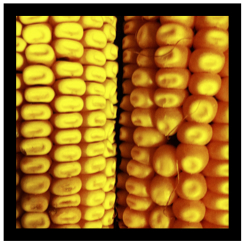
\includegraphics[width=.8\linewidth]{Figures/corn.jpg}
\caption{Placeholder image of corn with a long example caption to show justification setting.}
\label{fig:computerNo}
\end{figure}


Figure \ref{fig:computerNo} shows an example of how to insert a column-wide figure. To insert a figure wider than one column, please use the \verb|\begin{figure*}...\end{figure*}| environment. Figures wider than one column should be sized to 11.4 cm or 17.8 cm wide. Use \verb|\begin{SCfigure*}...\end{SCfigure*}| for a wide figure with side captions.

\section*{Conclusions}

\lipsum[3-3]
 \ref{fig:computerNo}

\subsection*{Corn}
\lipsum[1-2]

\section*{Conclusions}
\lipsum[6-6]


 \ref{fig:computerNo}

\begin{acknowledgements}
Felix Andrews
\end{acknowledgements}

\section*{Bibliography}
\bibliography{biblio}

%% You can use these special %TC: tags to ignore certain parts of the text.
%TC:ignore
%the command above ignores this section for word count
\onecolumn
\newpage

\section*{Word Counts}
This section is \textit{not} included in the word count.

\subsection*{Statistics on word count}
\detailtexcount
\newpage

%%%%%%%%%%%%%%%%%%%%%%%%%%%%%
% Supplementary Information %
%%%%%%%%%%%%%%%%%%%%%%%%%%%%%
\captionsetup*{format=largeformat}
\section{Supplemental Information} \label{note:Note1}
\lipsum[3-3]
%TC:endignore
%the command above ignores this section for word count

\end{document}
